\documentclass[dvipsnames, aspectratio=43] {beamer}

\if 0
%\usepackage{latex_templates/beamerthemeMSP}
\usepackage{wasysym}
\usepackage{pifont}% http://ctan.org/pkg/pifont
\newcommand{\cmark}{{\color{textColor}\ding{51}}}%
\newcommand{\xmark}{{\color{textColor}\ding{55}}}%
\newcommand{\nmark}{{\color{textColor}\ding{51}\ding{55}}}%
\fi

\usepackage{cmlgc}
\usepackage{comment}
\usepackage{tikz}
\usefonttheme{serif}     % Font theme: serif
\usepackage[T2A]{fontenc}
\usepackage[utf8]{inputenc}
\usepackage[english]{babel}
\usepackage{amssymb,amsfonts,amsmath,mathtext,cite,enumerate,float} %подключаем нужные пакеты расширений
% \usepackage{cyrillic}
\usepackage{color, colortbl}
\usepackage{multirow}
\usepackage{graphicx}
\usepackage{graphics}
\usepackage{multirow}
\usepackage{url}
\usepackage{hyperref}
\usepackage{animate}
\usepackage{pifont}
\usepackage{wasysym}
\usepackage{marvosym}
\usepackage{appendixnumberbeamer} 
\usepackage{pgfpages}
\usepackage{systeme,mathtools}
\usepackage{mathtools}
\usepackage{listings}
\usepackage{xcolor} % for setting colors
\usepackage{mhchem}
\usepackage{epstopdf}

\usepackage{ragged2e} %выравнивание текста по ширине слайда (\justifying)
%\setbeamercolor{background canvas}{bg=violet}


\usetheme{Madrid}
\usecolortheme{dove}
%=================================================

\defbeamertemplate*{footline}{mytheme}{%
  \leavevmode%
  \hbox{%
    \begin{beamercolorbox}[wd=.2\paperwidth,ht=3ex,dp=1ex,center]{author in head/foot}%
      \usebeamerfont{author in head/foot}\insertshortauthor
    \end{beamercolorbox}%
    \begin{beamercolorbox}[wd=.7\paperwidth,ht=3ex,dp=1ex,center]{title in head/foot}%
      \usebeamerfont{title in head/foot}\insertshorttitle
    \end{beamercolorbox}%
    \begin{beamercolorbox}[wd=.1\paperwidth,ht=3ex,dp=1ex,right]{date in head/foot}%
      %\usebeamerfont{date in head/foot}\insertshortdate{}\hspace*{2em}
      %\insertframenumber{} / \inserttotalframenumber\hspace*{2ex} %номер текущего слайда / общее число слайдов
      \insertframenumber{} \hspace*{5ex}  %номер текущего слайда
  \end{beamercolorbox}}%
  \vskip0pt%
}
\usebeamertemplate{mytheme}
\beamertemplatenavigationsymbolsempty

\defbeamertemplate*{frametitle}{boldTitle}{%
  \begin{beamercolorbox}[wd=\paperwidth,ht=3ex,dp=3pt,center]{title in head/foot}%
    %        \ \textit{\textbf{\insertframetitle}} % курсивный заголовок слайда 
    \ \textbf{\insertframetitle}
  \end{beamercolorbox}
}
\usebeamertemplate{boldTitle}
\setbeamercovered{dynamic}

\setbeameroption{hide notes} % Only slides
%\setbeameroption{show only notes} % Only notes
%\setbeameroption{show notes on second screen=right} % Both
%\setbeamertemplate{note page}[plain]


%=================================================
% \titlegraphic{\includegraphics[width=\textwidth]{logo_conf.png}}

%\addtobeamertemplate{title page}{\centering \includegraphics[scale=0.2]{logos.png}}{}
\addtobeamertemplate{title page}{\centering \includegraphics[scale=0.31]{baldin_Logo_2018n.png}}{}
\addtobeamertemplate{title page}{\centering \includegraphics[scale=.05]{bmn_logo.png}}{} 
%\addtobeamertemplate{title page}{\centering \includegraphics[scale=0.095]{wpcf2018/wpcf2018_2.png}}{}

\title[\bf The XXIV International Baldin Seminar on High Energy Physics Problems]{\textbf{\large {Event reconstruction in the BM@N experiment}}}

%\author[P.~Batyuk]{\textit{\textbf{{\footnotesize \underline{P.~Batyuk}, L.~Malinina (SINP MSU, JINR), \\ O.~Rogachevskiy (JINR)}}} \\
%  on behalf of the MPD collaboration}
\author[\bf P.~Batyuk]{\textit{\textbf{{\footnotesize \underline{P.~Batyuk} on behalf of software group}}}} 
%on behalf of the MPD collaboration} 
\institute{\bf Dubna, Joint Institute for Nuclear Research}
\vskip -.3cm
\date{{\textbf{NICA/MPD parallel session, September 19}}}  
% \newpage \footnotesize April 14, 2016}}

\lstset{
  %    frame=tb, % draw a frame at the top and bottom of the code block
  tabsize=4, % tab space width
  showstringspaces=false, % don't mark spaces in strings
  %   numbers=left, % display line numbers on the left
  commentstyle=\color{blue}, % comment color
  keywordstyle=\color{blue}, % keyword color
  stringstyle=\color{red} % string color
}

\graphicspath{{../common_figures/}}

\begin{document}
\maketitle

\begin{frame}
  \bf
  \frametitle{\bf \centering Outline}
  \begin{itemize}
  \item BM@N experiment and its physics motivation
  \item Geometry description
  \item Inner tracker and a new version of tracking procedure
  \item Alignment of inner tracker
  \item Event visualization
  \item Conclusion
  \end{itemize}
\end{frame}

\begin{frame}
  \frametitle{\bf \centering BM@N experiment}
  \bf
       \vskip -.35cm
       \begin{columns}[c]
         \column{.69\textwidth}
         \begin{block}{\bf \centering Full setup, layout}
           \begin{figure}[H]
             \includegraphics[width=1.\linewidth]{bmn_full_config_color_detectors_moreDarkMagnet_without_straw_labels.png}
           \end{figure}
         \end{block}

         \column{.29\textwidth}
         {\tiny
           \begin{block}{}
             \begin{itemize}
             \item Central tracker (Silicon tracker + GEM) inside analyzing magnet to reconstruct
               AA-interactions
             \item Outer tracker (CPC, DCH) behind magnet to link tracks from central tracker to ToF detectors
             \item TOF1 \& TOF2 system based on mRPC and T0 detectors to identify hadrons and light nuclei
             \item Detectors to form T0 and beam monitors
             \item ZDC calorimeter to measure centrality of AA-collisions
             \item Electromagnetic calorimeter for $\gamma$, $e^{+}$, $e^{-}$
             \end{itemize}
           \end{block}
         }
       \end{columns}
       \vskip -.2cm
       {\footnotesize
         \begin{block}{\bf \centering {\scriptsize  BM@N advantages:}}
           \vskip -.1cm
         \begin{itemize}
         \item \centering large aperture analyzing magnet
         \item sub-detector systems are resistant to high multiplicities of charged particles
         \item PID: "near to magnet" (TOF1), "far from magnet" (TOF2)
         \end{itemize}
       \end{block}
       }
\end{frame}

\begin{frame}
  \bf
  \frametitle{\bf \centering QCD phase diagram}
  \vskip -.75cm
  \begin{columns}[t]
    \column{.49\textwidth}
    \begin{block}{}
      \begin{figure}[H]
        \includegraphics[width=1.\linewidth]{qcd_diagram.png}
      \end{figure}
    \end{block}
    \vskip -.75cm

    \begin{columns}[t]
      \column{.48\textwidth}  
      \begin{block}{\bf \centering {\tiny High energy:}}
        {\tiny
          \begin{itemize}
          \item $N_{baryons} \approx N_{antibaryons}$
          \item Lattice QCD predicts crossover transition between hadronic and partonic matter
          \item ALICE, ATLAS, CMS, STAR, PHENIX
          \end{itemize}
        }
      \end{block}
      \column{.48\textwidth}
      \begin{block}{\bf \centering {\tiny High net-baryon density:}}
        {\tiny
          \begin{itemize}
          \item $N_{baryons} >> N_{antibaryons}$
          \item Lattice QCD not applicable, models predict structures and exotic phases 
          \item BES @ RHIC, NA61, CBM, {\color{red} NICA/MPD, BM@N}
          \end{itemize}
        }
      \end{block}
    \end{columns}

    \column{.48\textwidth}
    \begin{block}{\bf \centering  Landscape of experiments exploring QCD phase diagram}
      \vskip .25cm
      \begin{figure}[H]
        \includegraphics[width=1.\linewidth]{QCD_dense_matter_experiments.png}
      \end{figure}
    \end{block}
  \end{columns}
  \note{One of the most urgent task for the study of the QCD phase diagram is density frontier.
    According to various calculations maximum freeze-out density is reached at the energy range around $\sqrt{s_{NN}}$ = 10 GeV/n.
    So, NICA is well suited for exploring the transition between the hadronic and quark-gluon phases at the high net-baryon
    density. This is the top priority of the NICA program. \\
    The landscape of HIC experiments, present and future, in the energy
    region of max baryonic density are presented in this figure. Among fixed target experiments
    CBM at FAIR will provide maximum interaction rate. There are only two collider experiments – NICA and STAR BES with
    a difference in interaction rate of 3-4 orders of magnitude. Two NICA experiments - BM@N with fixed target and MPD
    at the collider will cover the whole indicated energy region.
  }
\end{frame}

\begin{frame}
  \bf
  \frametitle{\bf \centering {\footnotesize Exploring high density baryonic matter with Nuclotron}}
  \vskip -.75cm
  \begin{columns}[t]
    \column{.51\textwidth}
    \begin{block}{}
      \includegraphics[width=1.\linewidth]{bar_densities.png}
    \end{block}
    \column{.47\textwidth}
       \begin{block}{}
         \includegraphics[width=1.\linewidth]{barDensDomination.png}
       \end{block}
\end{columns}
  \begin{block}{}
    \begin{center}
      Nuclotron is well suited to study high density (dominantly baryonic) matter since at that energies
      baryon-dominated system exists comparatively long lifetime
    \end{center}
  \end{block}
\end{frame}

\begin{frame}
  \frametitle{\bf \centering BM@N experiment at previous runs}
  \vskip -.75cm
  \begin{columns}[t]
    \column{.69\textwidth}
    \begin{block}{\bf \centering Experimental setup at deuteron and carbons runs}
      \includegraphics[width=1.\linewidth]{bmn_winter2016_config_common_view_labels.png}
    \end{block}
  \end{columns}
  \begin{columns}[t]
    \column{.37\textwidth}
    \begin{block}{}
      \includegraphics[width=1.\linewidth]{rigidity_1800A_run6.png}
    \end{block}
    \column{.27\textwidth}
    \begin{block}{}
      \includegraphics[width=1.\linewidth]{momBeam_run6.png}
    \end{block}
    \column{.27\textwidth}
    \begin{block}{}
      \includegraphics[width=1.\linewidth]{momResBeam_run6.png}
    \end{block}
  \end{columns}
\end{frame}

\begin{frame}
  \bf
  \frametitle{\bf \centering {\footnotesize BM@N and SRC, data collected in Ar/Kr run (RUN7)}}
  \vskip -.45cm
  \begin{columns}[c]
    \column{.49\textwidth}
    {\scriptsize
    \begin{block}{}
      SRC:
      \begin{itemize}
      \item One beam energy available for C-beam
      \item More than half of the collected statistics can be used for analysis
      \end{itemize}
      BM@N:
      \begin{itemize}
      \item One beam energy available for Ar-beam and three - for Kr-beam
      \item Wide set of targets used ($C, Al, Cu, Sn, Pb$)
      \end{itemize}
    \end{block}
    }
    \column{.50\textwidth}
    \begin{block}{\bf \centering SRC}
     \begin{figure}[H]
      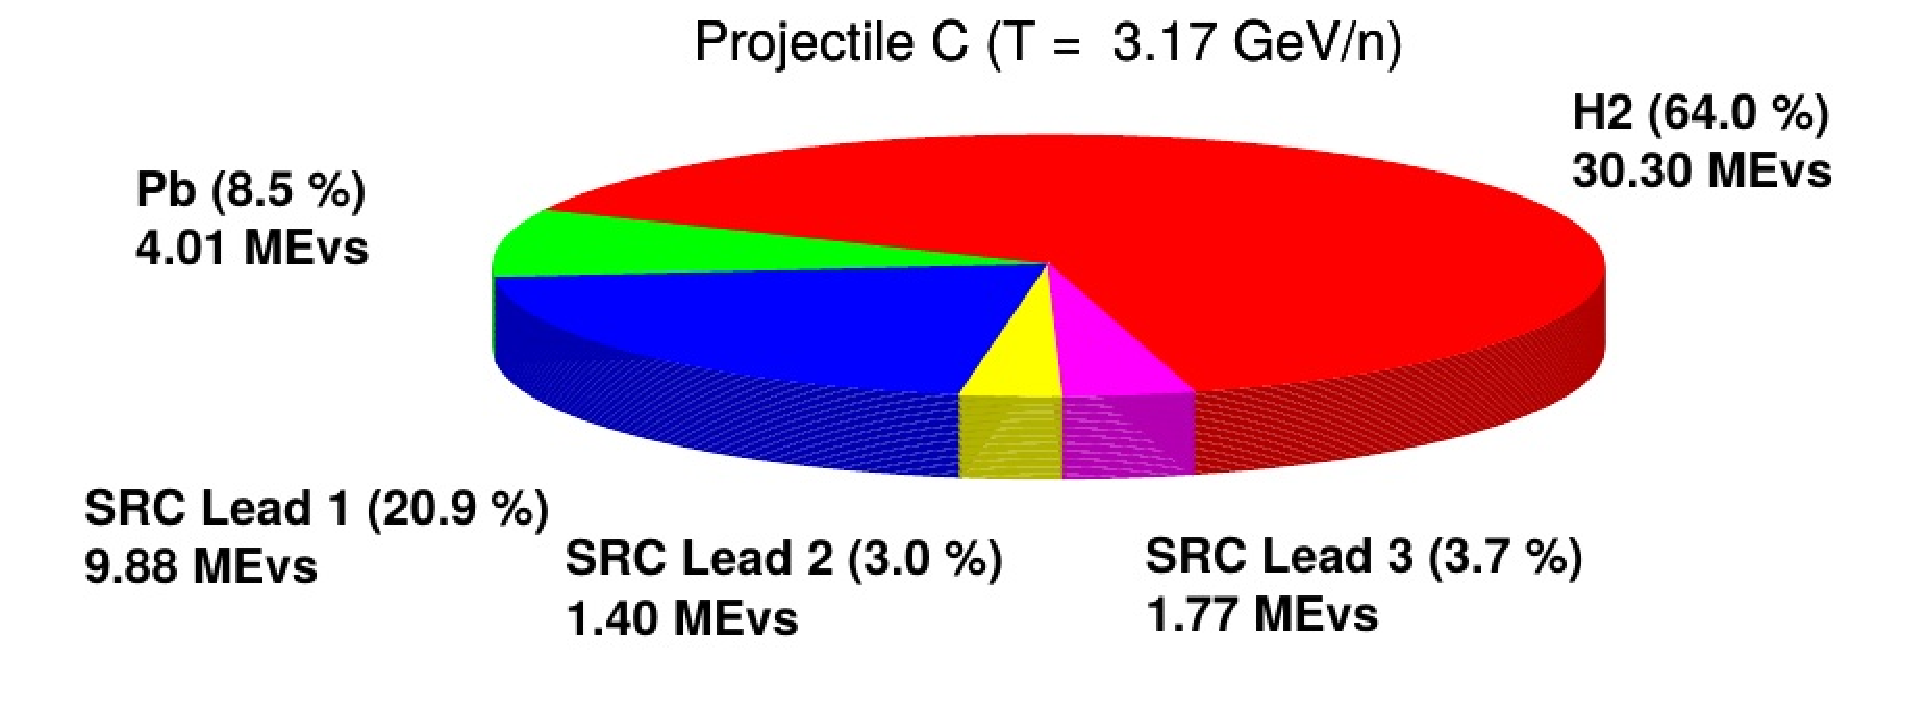
\includegraphics[width=1.\linewidth]{DataCollected_SRC_Run7}
    \end{figure}
    \end{block}
    \vskip -.2cm
  \end{columns}
  \vskip -.2cm
  \begin{block}{\bf \centering BM@N}
     \begin{figure}[H]
      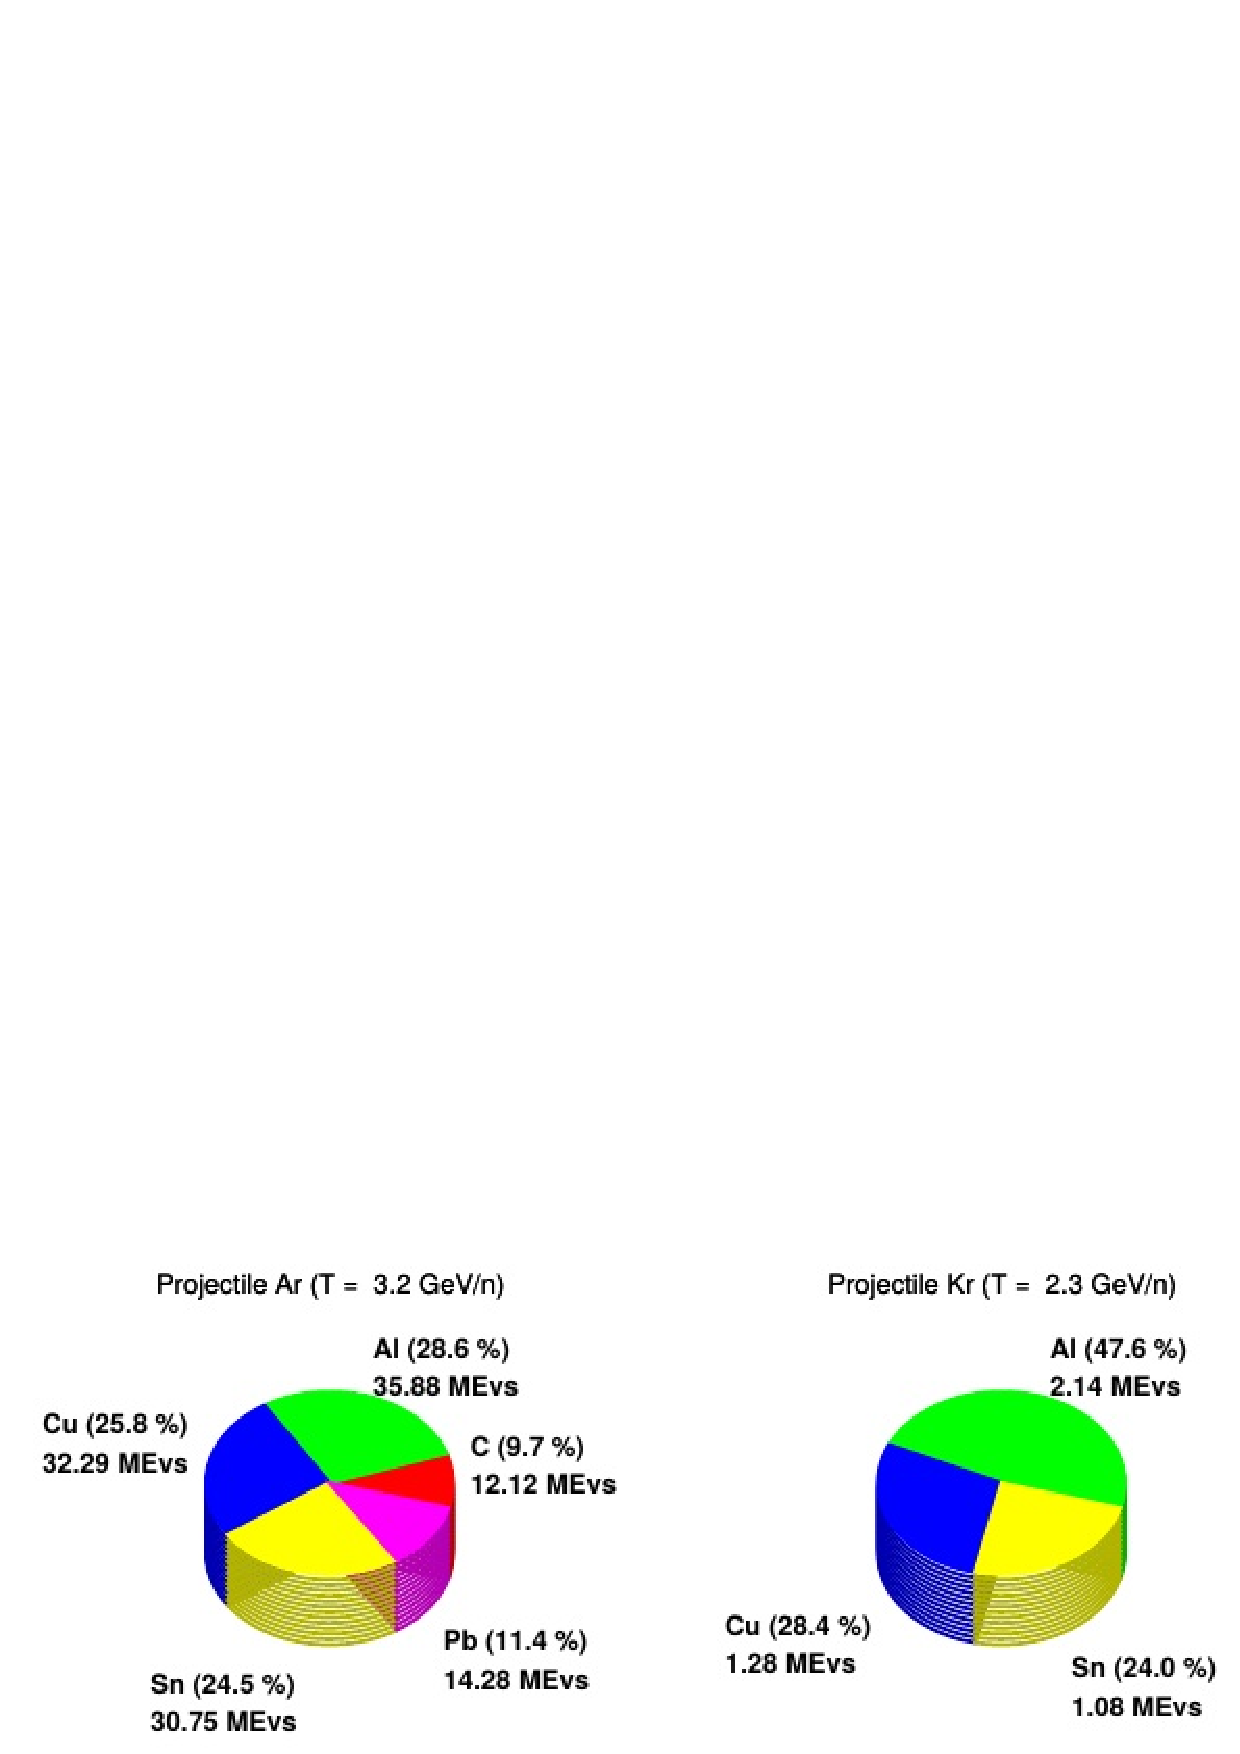
\includegraphics[width=1.\linewidth]{DataCollected_BMN_Run7.png}
    \end{figure}
  \end{block}
\end{frame}

\begin{frame}
  \bf
  \begin{block}{}
    \begin{center}
      {\Huge Hit reconstruction in strip detectors}
    \end{center}
  \end{block}
\end{frame}

\begin{frame}
  \bf 
  \frametitle{\bf \centering BM@N and SRC configurations @ RUN7}
  \vskip -.5cm
  \begin{columns}[t]
    \column{.49\textwidth}
    \begin{block}{ \bf \centering {\color{blue} SRC}}
         \includegraphics[width=1.\linewidth]{src_RUN7.png}
    \end{block}
    \column{.49\textwidth}
    \begin{block}{\bf \centering {\color{red} BM@N}}
      \includegraphics[width=1.\linewidth]{bmn_RUN7.png}
    \end{block}
  \end{columns}
  \begin{block}{}
    {\scriptsize
    \begin{itemize}
    \item Inner tracker system consists of two subdetectors: GEM (Gas Electron Multiplier) and SILICON
    \item GEM detector is a set of gas-filled chambers functioning by a principle of gas electron multiplication.
    \item SILICON is a module semiconductor detector to be used for precise reconstruction of primary vertex in event. 
    \end{itemize}
    }
  \end{block}
\end{frame}

\begin{frame}
  \frametitle{\bf \centering Towards realistic simulation of GEM tracker}
  \vskip -.25cm
  \begin{block}{}
    \begin{center}
      \bf {\footnotesize Simulation of GEM response: Garfield++}
    \end{center}
  \end{block}
  \vskip -.75cm
  \begin{columns}[t]
    \column{.49\textwidth}
    {\scriptsize
    \begin{block}{}
      \bf
      \begin{itemize}
        \item {\color{red} Garfield++} is a framework for micro-simulation of physical processes in gas detectors 
        \item A charge particle passing through GEM chamber detecting volume ionizes electrons in gas  
        \item Multiplayer GEM-cascades form avalanches which drift to readout-plane and fire strips
      \end{itemize}
    \end{block}
    }
    \vskip -.4cm
    \begin{block}{\bf \centering {\scriptsize Simulation parameters in Garfield++}}
      \includegraphics[width=1.\linewidth]{GEM_internStruct.png} 
    \end{block}
    \column{.49\textwidth}
    \begin{block}{\bf \centering {\scriptsize Structure of BM@N GEM chamber and simulated electron avalanches}}
      \includegraphics[width=1.\linewidth]{GEM_electronAvalanche.png} 
    \end{block}
    \vskip -.3cm
    \begin{block}{\bf \centering {\scriptsize Profile of electron avalanche at the readout-plane (cluster)}}
      \includegraphics[width=1.\linewidth]{GEM_electronAvProfile.png} 
    \end{block}
  \end{columns} 
\end{frame}

\begin{frame}
  \bf
  \vskip -.7cm
  \frametitle{\bf \centering Towards realistic simulation of GEM tracker}
  \begin{columns}[t]
    \column{.49\textwidth}
    \begin{block}{}
      \bf \centering Aim: to obtain a mean shift of electron clusters (Lorentz shift) as a function of magnetic field and gas mixture ($ArCO_{2}$, $ArC_{4}H_{10}$)
    \end{block}
    \begin{block}{}
      \begin{itemize}
     % \item Aim: to obtain a mean shift of electron clusters (Lorentz shift) as a function of magnetic field and gas mixture ($ArCO_{2}$, $ArC_{4}H_{10}$)
      \item {\color{red} Lorentz shift has a tendency to increase with increasing of magnetic field}
      \item {\color{blue} Taking into account Lorentz shift allows us to increase reconstruction efficiency}
      \end{itemize}
    \end{block}
    \column{.49\textwidth}
    \begin{block}{}
      \includegraphics[width=1.\linewidth]{lorShiftDep.png} 
    \end{block}
    \vskip -.3cm
     \begin{block}{\bf \centering All possible realistic effects to be included in simulation if necessary:}
       \begin{itemize}
       \item Lorentz shift
       \item Remain misalignment
       \item Detector inefficiency 
       \end{itemize}
    \end{block}
  \end{columns}
\end{frame}

\begin{frame}
  \frametitle {\bf \centering {\footnotesize Hit reconstruction in strip detectors}}
  \vskip -.9cm
  \begin{columns}[t]
    \column{.51\textwidth}
     % {\bf
      \begin{block}{} 
      \begin{enumerate}
      \item {\footnotesize \bf {\color{blue} Clusterization}}
        \begin{itemize}
        \item {\scriptsize Search for strip clusters is done by "peak-valley-peak" method for each strip layer}
        \item {\scriptsize Center of a found strip cluster is calculated by "center-of-gravity" method} 
        \end{itemize}
       \item {\footnotesize \bf {\color{red} Reconstruction}}
        \begin{itemize}
        \item {\scriptsize Real coordinates are being found when crossing all strips pertaining to each layer and using the center positions of previously found clusters}
        \item {\scriptsize Obtained intersections that belong to a strip layer we are considering are supposed to be ``hits''}
        \item {\scriptsize "Hits" we have found at the previuos step have a fraction of not only real ones ("fakes")} 
        \end{itemize}
      \end{enumerate}          
      \end{block}
    %  }
     
    \column{.44\textwidth}
    \begin{block}{}
      \vskip -.1cm
      \includegraphics[width=1.\linewidth]{stripHitReco.png}
    \end{block}
    \vskip -.4cm
    \begin{block}{}
        \vskip -.2cm
    %  {\bf \centering {\tiny Number of "fakes'' can be decreased by decreasing angle between strips in two readout planes (upper and lower layers)}
      \includegraphics[width=1.\linewidth]{fakes_description.png}
      \vskip -.3cm
      {\scriptsize \bf Number of "fakes'' can be decreased by decreasing angle between strips in two readout planes (upper and lower layers)}
    \end{block}    
  \end{columns}
\end{frame}

\begin{frame}
  \bf
  \begin{block}{}
    \begin{center}
      {\Huge Tracking}
    \end{center}
  \end{block}
\end{frame}

\begin{frame}
  \bf
  \frametitle{\bf \centering CellAutoTracking, \underline{algorithm}}
  \vskip -.75cm
  \begin{columns}[t]
    \column{.49\textwidth}
    \begin{block}{}
      \begin{itemize}
      \item Based on cellular automaton
      \item Applicable to inner tracker (GEM and silicon hits simultaneously)
      \end{itemize}
    \end{block}
     \begin{block}{\bf \centering {\tiny Inner tracker configuration}}
      \includegraphics[width=1.\linewidth]{TrackingScheme_stations.pdf}
     \end{block}
    \column{.49\textwidth}   
      \begin{block}{\bf \centering {\tiny Hits in inner tracker}}
      \includegraphics[width=1.\linewidth]{TrackingScheme_hits.pdf}
      \end{block}
      \begin{block}{\bf \centering To get more, see:}
        R. Glattauer, R. Fr\"{u}hwirth, J. Lettenbichler and W. Mitaroff \\
        \centering {\color{red} arXiv:1202.2761}
      \end{block}
  \end{columns}
\end{frame}

\begin{frame}
  \frametitle{\bf \centering CellAutoTracking, \underline{creation of cells}}
  \bf
   \vskip -.75cm
  \begin{columns}[t]
    \column{.49\textwidth}
    \begin{block}{\bf \centering {\footnotesize 1. ``All-to-all'' connection}}
      \includegraphics[width=1.\linewidth]{TrackingScheme_cells.pdf}
    \end{block}
    
    \column{.49\textwidth}
    \begin{block}{\bf \centering {\footnotesize 2. Remove cells with big slopes}}
      \includegraphics[width=1.\linewidth]{TrackingScheme_cells_slopeSelection.pdf}
    \end{block}
  \end{columns}   
\end{frame}

\begin{frame}
  \frametitle{\bf \centering CellAutoTracking, \underline{calculation of states}}
   \bf
   \vskip -.75cm
  \begin{columns}[t]
    \column{.33\textwidth}
    \begin{block}{\bf \centering Loop over cells:}
      \begin{itemize}
      \item All cells have a zero-state in the beginning
      \item If a left neighbour {\color{red} has the same state} and {\color{red} common hit with current cell} $\rightarrow$
        state of current cell is increased by 1
      \end{itemize}
    \end{block}
    \column{.31\textwidth}
    \begin{block}{\bf \centering Iteration 1}
      \includegraphics[width=1.\linewidth]{TrackingScheme_cells_state1.pdf}
    \end{block}
    \begin{block}{\bf \centering Iteration 5}
      \includegraphics[width=1.\linewidth]{TrackingScheme_cells_state5.pdf}
    \end{block}
    
    \column{.31\textwidth}
    \begin{block}{\bf \centering Iteration 3}
      \includegraphics[width=1.\linewidth]{TrackingScheme_cells_state3.pdf}
    \end{block}
    \begin{block}{\bf \centering Iteration 7}
      \includegraphics[width=1.\linewidth]{TrackingScheme_cells_state7.pdf}
    \end{block}
  \end{columns}
\end{frame}

\begin{frame}
  \frametitle{\bf \centering CellAutoTracking, \underline{connection of cells}}
  \bf
  \vskip -.8cm
  \begin{columns}[t]
    \column{.33\textwidth}
    \begin{block}{\bf \centering {\tiny Last iteration}}
      \vskip -.2cm
      \includegraphics[width=1.\linewidth]{TrackingScheme_cells_state7.pdf}
      \vskip -.3cm
      {\scriptsize Loop over cells in backward direction:}
  % \end{block}
    \vskip -.3cm
  %  \begin{block}{\bf \centering {\scriptsize Loop over cells in backward direction:}}
       \begin{itemize}
       \item {\scriptsize {\color{blue} Left neighbour has a less state than current one}}
       \item {\scriptsize {\color{blue} Difference between its slope and slope of current cell is minimal for all left neighbours}}
       \item {\scriptsize {\color{blue} Left neighbour is in validation gate}}
       \end{itemize}
    \end{block}
    \column{.31\textwidth}
    \begin{block}{\bf \centering {\tiny 1. Creation of \\ candidates}}
      \includegraphics[width=1.\linewidth]{TrackingScheme_cells_connection.pdf}
    \end{block}
    \begin{block}{\bf \centering {\tiny 3. Remove short cand. with $N_{shared} > 0$}}
      \includegraphics[width=1.\linewidth]{TrackingScheme_track_selection_by_SharedHits.pdf}
    \end{block}
    \column{.31\textwidth}
    \begin{block}{\bf \centering {\tiny 2. Remove candidates with $N_{hits} < 4$}}
      \includegraphics[width=1.\linewidth]{TrackingScheme_cells_selection_by_nHits.pdf}
    \end{block}
    \begin{block}{\bf \centering {\tiny 4. Refit candidates by Kalman Filter}}
      \includegraphics[width=1.\linewidth]{TrackingScheme_track_refit.pdf}
    \end{block}
  \end{columns}
\end{frame}

\begin{frame}
  \bf
  \frametitle{\bf \centering CellAutoTracking, \underline{input for QA}}
  \begin{block}{}
    \begin{itemize}
      \item Inner tracker data, RUN7 geometry used
      \item Generator: LAQGSM, ArPb (T = 3.2 GeV/n), minbias, 10k events
      \item Magnetic field: B = 0 T and B = 0.59 T
      \item Mean multiplicity: 130
      \item Primary vertex: $V_{p}$ = (0.5, -4.6, -2.3)
    \end{itemize}
  \end{block}
  \begin{block}{}
    \includegraphics[width=1.\linewidth]{qa_input.pdf}
  \end{block}
\end{frame}

\begin{frame}
  \bf
  \frametitle{\bf \centering CellAutoTracking, \underline{quality assurance (QA)}}
  \vskip -.8cm
  \begin{columns}[t]
    \column{.54\textwidth}
    \begin{block}{\bf \centering Efficiency}
      \includegraphics[width=1.\linewidth]{efficiency.png}
    \end{block}
    \column{.44\textwidth}
    \begin{block}{}
     % \begin{itemize}
     % \item
      \begin{itemize}
      \item {\tiny \alert{Efficiency}: $\frac{N_{well} - N_{split}}{N_{MC}} \cdot 100\%$}
      \item {\tiny \alert{Percent of ghosts}: $\frac{N_{wrong}}{N_{rec}} \cdot 100\%$}
      \item {\tiny \alert{Percent of clones}: $\frac{N_{split}}{N_{rec}} \cdot 100\%$}
      \item {\tiny {\color{blue} $N_{MC}$} is a set of Monte Carlo tracks (MC-tracks)
        with more than 3 hits in inner tracker}
      \item {\tiny {\color{blue} $N_{rec}$} is a set of all reconstructed tracks}
      \item {\tiny {\color{blue} $N_{well}$} is a sample of reconstructed tracks where
        each track has \underline{more} than 60\% of hits that correspond to the same MC-track}
      \item {\tiny {\color{blue} $N_{wrong}$} is a sample of reconstructed tracks where
        each track has \underline{less} than 60\% of hits that correspond to the same MC-track}
      \item {\tiny {\color{blue} $N_{split}$} is a number of reconstructed tracks corresponding
        to the same MC-track}
      \end{itemize}
      % \end{itemize}
    \end{block}
  \end{columns}
\end{frame}

\begin{frame}
  \bf
  \frametitle{\bf \centering CellAutoTracking, \underline{QA}}
 % \vskip -.75cm
  \begin{columns}[c]
    \column{.5\textwidth}
    \begin{block}{\bf \centering Momentum resolution}
      \includegraphics[width=1.\linewidth]{momRes_yesField_noSil.png}
    \end{block}
    \begin{block}{}
      \includegraphics[width=1.\linewidth]{momRes_yesField_yesSil.png}
    \end{block}
    \column{.4\textwidth}
    \begin{block}{\bf \centering {\color{red} Use of silicon:}}
      \begin{itemize}
      \item Allows one to obtain un unbiased estimate for all values of momentum in a wide range
      \item Improves mom. resolution, especially at high momenta 
      \end{itemize}
    \end{block}
  \end{columns}
\end{frame}

\begin{frame}
  \bf
  \frametitle{\bf \centering CellAutoTracking, \underline{QA}}
  \vskip -.75cm
  \begin{columns}[t]
    \column{.49\textwidth}
    \begin{block}{\bf \centering Primary vertex}
      \includegraphics[width=1.\linewidth]{vertZ_noField.pdf}
    \end{block}
    \begin{block}{}
      \includegraphics[width=1.\linewidth]{vertZ_yesField.pdf}
    \end{block}
    \column{.49\textwidth}
    \begin{block}{}
      {\footnotesize Primary vertex is reconstructed by \\ {\color{red} method of virtual planes}}
    \end{block}
    \begin{block}{}
      \begin{itemize}
      \item {\footnotesize Use of silicon leads to a more precise reconstruction of primary vertex $V_{p}$}
      \item {\footnotesize Effect becomes significant when reconstructing tracks in magnetic field}
      \end{itemize}
    \end{block}
    \begin{block}{\bf \centering Vertex efficiency}
      \resizebox{\columnwidth}{!}{%
        {\footnotesize 
        \begin{tabular}{| c | c | c|}
          \hline
	  %\cline{2-3}
          \multirow{2}{*}{$B_{y}$ [T]} & \multicolumn{2}{c|}{SILICON} \\
          \cline{2-3}
          & On & Off \\
          \hline
          0.0 & 64\% & 64\% \\
          \hline
          {\color{red} 0.59} & {\color{red} 54 \%} & {\color{red} 49\%} \\
          \hline
        \end{tabular}
        }
      }
    \end{block}
  \end{columns}
\end{frame}

\begin{frame}
  \bf
  \begin{block}{}
    \begin{center}
      {\Huge Alignment}
    \end{center}
  \end{block}
\end{frame}

\begin{frame}
  \bf
  \vskip -.35cm
  \frametitle{\bf \centering Alignment}
  \begin{block}{}
    The package based on formalism of {\color{red} Millepede II} with all its features and allows one to include / exclude different
    subdetectors from alignment (GEM, silicon).
  \end{block}
  \begin{block}{\bf \centering {\color{blue} Generalized straight-line model of track:}}
    \vskip -.5cm
    \begin{equation*}
      u^{j}_{i} = x_{0}^{j} \cos \alpha_{i} + t_{x}^{j} \cos \alpha_{i} + y_{0}^{j} \sin \alpha_{i} + t^{j}_{y} z \sin \alpha_{i} +
      \Delta u_{i} + (t_{x} \cos \alpha_{i} + t_{y} \sin \alpha_{i}) \Delta z 
    \end{equation*}
  \end{block}
  \vskip -.7cm
  \begin{columns}[t]
    \column{.49\textwidth}
    \begin{block}{\bf \centering Chosen weights to prevent det. shift:}
      \begin{itemize}
      \item $w_{i}^{1} = \cos \alpha_{i}$ - shifts ($x_{0}$)
      \item $w_{i}^{2} = z_{i} \cos \alpha_{i}$ - shearings ($t_{x}$)
      \item $w_{i}^{3} = \cos \alpha_{i}$ - shifts ($y_{0}$)
      \item $w_{i}^{4} = z_{i} \sin \alpha_{i}$ - shearings ($t_{y}$)
      \item $w_{i}^{5} = 1$ - overall shift in Z
      \item $w_{i}^{6} = z_{i}$ - scaling in Z
      \end{itemize}
    \end{block}
    \column{.49\textwidth}
    \begin{block}{\bf \centering {\footnotesize Misaligned and aligned detector}}
      \vskip -.1cm
      \includegraphics[width=1.\linewidth]{misAlignAndAlignedDet.pdf}
    \end{block}
    \vskip -.1cm
    \begin{block}{\bf \centering {\footnotesize Also solutions but not desirable}}
      \vskip -.1cm
      \includegraphics[width=1.\linewidth]{alsoPossibleSolutions.pdf}
    \end{block}
  \end{columns}
\end{frame}

\begin{frame}
  \bf
  \frametitle{\bf \centering Test of alignment, RUN7}
  % \vskip -.75cm
  \begin{block}{}
    \begin{itemize}
    \item Ar + C(Cu, Al, Sn, Pb) $\rightarrow$ X without magnetic field (more than 10000 kEvents used)
    \item Set of all possible trigger conditions used
    \end{itemize}
  \end{block}
  \begin{columns}[c]
    \column{.31\textwidth}
    \begin{block}{\bf \centering Vertex (only GEM)}
      \includegraphics[width=1.\linewidth]{VpZ_corr.png}
    \end{block}
    \column{.31\textwidth}
    \begin{block}{\bf \centering Positions of detectors}
      \includegraphics[width=1.\linewidth]{si_scheme.png}
    \end{block}
    \column{.31\textwidth}
    \begin{block}{\bf \centering Residuals in GEM}
       \includegraphics[width=1.\linewidth]{alignResid.pdf}
    \end{block}
  \end{columns}
\end{frame}

\begin{frame}
  \bf
  \begin{block}{}
    \begin{center}
      {\Huge Event visualization}
    \end{center}
  \end{block}
\end{frame}

\begin{frame}
  \bf
  \vskip -.8cm
  \frametitle{\bf \centering Data processing for offline Event Display}
  \begin{columns}[t]
    \column{.3\textwidth}
    \begin{block}{\bf \centering {\footnotesize Sim \& Reco}}
      \vskip -.2cm
      \includegraphics[width=1.\linewidth]{offline_anal.png}
    \end{block}
    \vskip -.4cm
    \begin{block}{\bf \centering {\footnotesize Reco}}
      \vskip -0.2cm
      \includegraphics[width=1.\linewidth]{offline_anal_v2.png}
    \end{block}
    
    \column{.59\textwidth}
    \begin{block}{}
      %\vskip -.2cm
      \includegraphics[width=1.\linewidth]{eventDisplay_run6_v2.png}
     % \vskip -.2cm
   % \end{block}
   % \begin{block}{}
    %  \includegraphics[width=1.\linewidth]{eventDisplay_run6_v3.png}
    \end{block}
    \vskip -.4cm
    {\footnotesize 
    \begin{block}{}
      \begin{itemize}
      \item The Event Display has been developed for graphical representations of the NICA experiments in offline as well as online mode and integrated into the
        BmnRoot software.
      \item The visualization system gives an opportunity to visually check the developed algorithms for reconstruction and physical analysis of data.
      \end{itemize}
    \end{block}
    }
  \end{columns}
\end{frame}


\begin{frame}
  \bf
  \frametitle{\bf \centering Conclusion}
  \begin{block}{}
    \begin{itemize}
    \item Instruments and algorithms to be used for description of detector geometry,
      alignment procedure in automatic mode, hit production in strip detectors (GEM, silicon), event visualization
      already developed and can be used.
    \item Feasibility study with Monte Carlo input performed with new tracking showed good QA-results,
      thus allowing one to use the tracking when real experimental data processing.
    \end{itemize}
  \end{block}
  \begin{block}{}
    \centering Thank you for your attention!
  \end{block}
\end{frame}

\end{document}
